\documentclass{report_template_oxford}
\usepackage{pgfplots}
\pgfplotsset{compat=1.18}
\usepackage{glossaries}
\usepackage{float}
\usepackage{parskip}
\usepackage{hyperref}

%Acronyms 
\newacronym{yolo}{YOLO}{You Only Look Once}
\newacronym{3yp}{3YP}{Third-Year Project}
\newacronym{cgs}{CGS}{Central Ground Server}
\newacronym{tcn}{TCN}{Temporal Convolutional Network}
\newacronym{lstm}{LSTM}{Long Short-Term Memory}
\newacronym{cnn}{CNN}{Convolutional Neural Network}
\newacronym{rnn}{RNN}{Recurrent Neural Network}
\newacronym{gpu}{GPU}{Graphics Processing Unit}
\newacronym{mse}{MSE}{Mean Squared Error}
\newacronym{oosm}{OOSM}{Out Of Sequence Measurement}
\newacronym{ssm}{SSM}{State Space Model}
\newacronym{hud}{HUD}{Heads-Up Display}
\newacronym{map}{mAP}{Mean Average Precision}
\newacronym{nms}{NMS}{Non-Maximum Supression}
\newacronym{mot}{MOT}{Multiple-Object Tracking}
\newacronym{api}{API}{Application Programming Interface}
\newacronym{pads}{PADS}{Police Array Drone System}
\newacronym{botsort}{BoT-SORT}{Bag of Tricks for SORT}
\newacronym{reid}{ReID}{Re-Identification}
\newacronym{iou}{IoU}{Intersection over Union}
\newacronym{cmc}{CMC}{Camera Motion Compensation}
\newacronym{fps}{FPS}{Frames Per Second}
\newacronym{assoca}{AssocA}{Association Accuracy}
\newacronym{deta}{DetA}{Detection Accuracy}
\newacronym{mota}{MOTA}{Multiple Object Tracking Accuracy}
\newacronym{hota}{HOTA}{Higher Order Tracking Accuracy}
\newacronym{idsw}{IDSW}{Identity Switches}
\newacronym{gt}{GT}{Ground Truth}
\newacronym{tp}{TP}{True Positive}
\newacronym{hmi}{HMI}{Human Machine Interface}
\newacronym{rcnn}{R-CNN}{Region-based Convolutional Neural Networks}
\newacronym{rtt}{RTT}{Round-Trip Time}


\title{3YP report template}
\subtitle{Anything or empty}
\author{Kaito Bremner}
\date{March 2026}

\begin{document}
\maketitle

% Abstract
% - Concise summary of report
% - Naming of essential outcomes
% - As short as possible while providing key points
% - Less than 1 page
\pagenumbering{roman}
\newpage
\addcontentsline{toc}{section}{Abstract}
\fancyhead[C]{Kaito Bremner}
\section*{Abstract}

\lipsum[1]

\newpage
\fancyhead[C]{}
\tableofcontents

\newpage
\addcontentsline{toc}{section}{List of Figures}
\listoffigures

\newpage
\addcontentsline{toc}{section}{List of Tables}
\listoftables

\newpage
\addcontentsline{toc}{section}{Glossary}
\printglossaries

% Introduction
% - Provide background and motivation
% - Provide boundaries and goals to the project
% - Give a short overview of report structure
\newpage
\pagenumbering{arabic}
\fancyhead[C]{Kaito Bremner}
\section{Perception and visualisation}



\fancyhead[C]{Kaito Bremner}




\subsection{Introduction}
The perception and visualisation is system important to establish a method of converting aerial visual camera data from busy urban environments into an automated detection and tracking environment for operator interface. The ability for the system to accurately perceive and track a suspect determines how many criminals get caught and hence, how much crime can be reduced via this deterrent. The design and performance of the overall perception and visualisation architecture are considered in this section. 

\subsubsection{Key Objectives}
The key objective of this system is to gather and analyse multi-modal sensor data to be able to detect and track single or multiple suspects moving in an urban environment to display to a \gls{hmi}, using computer vision. The suspect(s) could be on-foot or travelling via car, motorycle and bicycle, hence the system aims to be able to cover all these cases. Finally, as discussed in Section [HMI] the operator will pick a single 'target' suspect to track, ensuring in multiple-suspect scenarios the individual drone remains in pursuit of at least a single suspect if the group splits up. This means the system should be able to detect with high recall, decent precision, and robust tracking accuracy, minimising the number of \gls{idsw}. As discussed in Section \ref{distributed}, the lack of onboard power and computational resources necessitates a more powerful corrective perception architecture run on the \gls{cgs}. The CGS must not only perceive the sensor data with higher fidelity, but more importantly, accurately predict suspect kinematics to account for edge-to-CGS network latency.

\subsubsection{Overview of design decision}
In the context of the \gls{pads} perception framework, the main constraints are real-time latency, edge-hardware limits (Section [Hardware]) and noisy environments. Overall, the system needs to be able to accurately detect and track a suspect's movements in dense urban environments from multi-modal sensor data. 

\textbf{Computer vision} \quad The system needs to be able to swiftly and accurately detect objects from live sensor feeds. Deep Learning (DL) based Computer Vision is the current industry standard for real-time object detection on drones using \glspl{cnn}, specifically the \gls{yolo} \cite{ultralytics_yolo26} architecture from Ultralytics, being used by 39.5\% of recent studies \cite{KATKURI2024100361}. \gls{yolo} is suitable for the detection of suspects in most urban environments, providing optimal computational speeds for edge deployment whilst matching the accuracy of bulkier architectures such as the \glspl{rcnn} \cite{DBLP:journals/corr/RedmonDGF15}, whilst also accurately dealing with occlusions and dense object scenarios. It also allows for the detection of multiple object classes, including vehicles. The most recent \gls{yolo}26 model series was chosen for its superior accuracy over previous models and is discussed further in Section \ref{distributed}.

\textbf{Tracking} \quad There are several tracking algorithms to ensure the system can identify and remember different suspects between frames in a sensor feed - \gls{botsort} is evaluated as the most suitable and tested in Section \ref{tracking}. 

\textbf{Cloud-based perception} \quad Although edge processing can provide somewhat accurate real-time sensor processing, it still produces inaccurate results. Ntousis et al. suggests '\textit{combining the relatively inaccurate results obtained by the limited hardware on the vehicle with those produced by a high-performance remote ground server, addressing the challenge of complex computations, namely detailed object detection, tracking, and approximate trajectory prediction ... in real time}'. There are several techniques to do this, in this case the \gls{lstm} was evaluated to perform the best for predictive compensation to overcome latency issues. This  \gls{cgs} architecture is further discussed in Section \ref{cloud based perception}. 

\textbf{Data Fusion} \quad This is important as \gls{pads} aims to be used for not only day-time but more often night-time situations, when burglary is more prevalent, so the implementation of sensors that can deal with both in Section [Hardware] is needed to boost perception accuracy in noisy environments. Late-stage and early-stage fusion methods exist for combining multi-modal data, but a method for combining four-way multi-modal data  does not yet exist. Section [data fusion] proposes a methodology to do this. 

\subsubsection{Overall System Framework}
\begin{enumerate}
    \item \textbf{Detection and Tracking} \quad Both the edge and \gls{cgs} systems use the \gls{yolo}v26 architecture to place bounding boxes around potential suspects with a 'class probability' confidence score on each frame (Section \ref{distributed}). Then the \gls{botsort} tracking algorithm is used to maintain consistent ID tags on objects between frames (Section \ref{tracking}). 
    \item \textbf{Data Fusion} \quad The \gls{cgs} conducts a combination of early and late-stage fusion to most accurately detect suspects in a video. (Section [data fusion]). 
    \item \textbf{Cloud-Based Perception} \quad The \gls{cgs} accounts for the latency arising from communication delays between the drone and base by using predictive compensation to predict target motion in the future, thereby synchronising the \gls{cgs} processed frame with the drone's real-time frame (Section \ref{cloud based perception}). This allows for real-time \gls{cgs} correction of the edge perception. 
    \item \textbf{Heads-Up Display} \quad This collective processing of the detection bounding box, tracking ID, next frame prediction is all overlaid into a final video feed (in the operator's chosen sensor type)  displayed to the operator interface as a \gls{hud} (Section \ref{hud}). 
\end{enumerate}



\subsection{Distributed perception} \label{distributed}
The need for distributed perception comes from the combination of limitations originating from the lack of onboard resources and latency between the \gls{cgs} and drone. [Alrik] calculates this latency at approximately 150ms, giving rise to the need for onboard edge perception, which allows for low latency automated decision making within drone. This comes at the cost of lower detection accuracy, and less robustness in handling edge cases, resulting from the need to use less complex \gls{yolo} models due to limited onboard compute. To counterbalance the drop in accuracy, a \gls{cgs} with compute to sustain a \gls{yolo} model with higher accuracy is implemented, aiding the onboard edge-perception despite latency issues. The specific methodology for implementing this cloud-perception architecture is discussed further in \ref{cloud based perception}. 

Keeping within the 20W power budget allocated in [Alrik's power budget section], the most novel \gls{yolo}v26 model series  was chosen for its higher \gls{map} when compared with older \gls{yolo} series, providing predictions directly without the need for \gls{nms}, a time-consuming post-processing technique for removing redundant overlapping detection boxes \cite{ultralytics_yolo26}. Specifically, the smallest YOLO26n was chosen for its smallest end-to-end latency compared to larger v26 models, an important consideration when inferencing in real time.

For the \gls{cgs}, the 2nd most complex \gls{yolo}26l was chosen for its superior \gls{map}, and near double increase in speed over the most accurate \gls{yolo}26x model, which only provides a marginal increase in \gls{map}.

\subsubsection{Training} \label{distributed_training}
AISKYEYE's VisDrone2019-DET \cite{visdrone2019} dataset was used for optimising the \gls{yolo}26n and \gls{yolo}26l on aerial imagery. The dataset consists of 6,471 training images, 548 validation images, and 1610 test images. The images are from the point of view of a drone with a focus on pedestrians and cars. For the \gls{pads} case, training only considered the people and pedestrian classes, as well as van, motorcycle, bicycle and car classes as potential getaway methods. The models were trained on Kaggle using Tesla 2 x T4 \glspl{gpu}, with the Adam optimiser over 100 epochs and a patience of 15 epochs. \gls{yolo}26n converged after 4 hours and 15 minutes, with per-image average processing times of 0.1ms preprocessing, 1.6ms inferencing and 0.2ms postprocessing. On the other hand, the \gls{yolo}26l converged after 10 hours and 35 minutes, stopping at the 89th epoch due to no improvements in accuracy after the 74th epoch. The average processing times were 0.1ms preprocessing, 8.7ms inferencing, and 0.2ms postprocessing per image. The \gls{yolo}26n's 81.6\% smaller inference time when compared with the \gls{yolo}26l is a reflection of its smaller complexity. 

\subsubsection{Results}
\begin{figure}[htbp]
    \centering
    \begin{minipage}{0.45\textwidth}
        \centering
        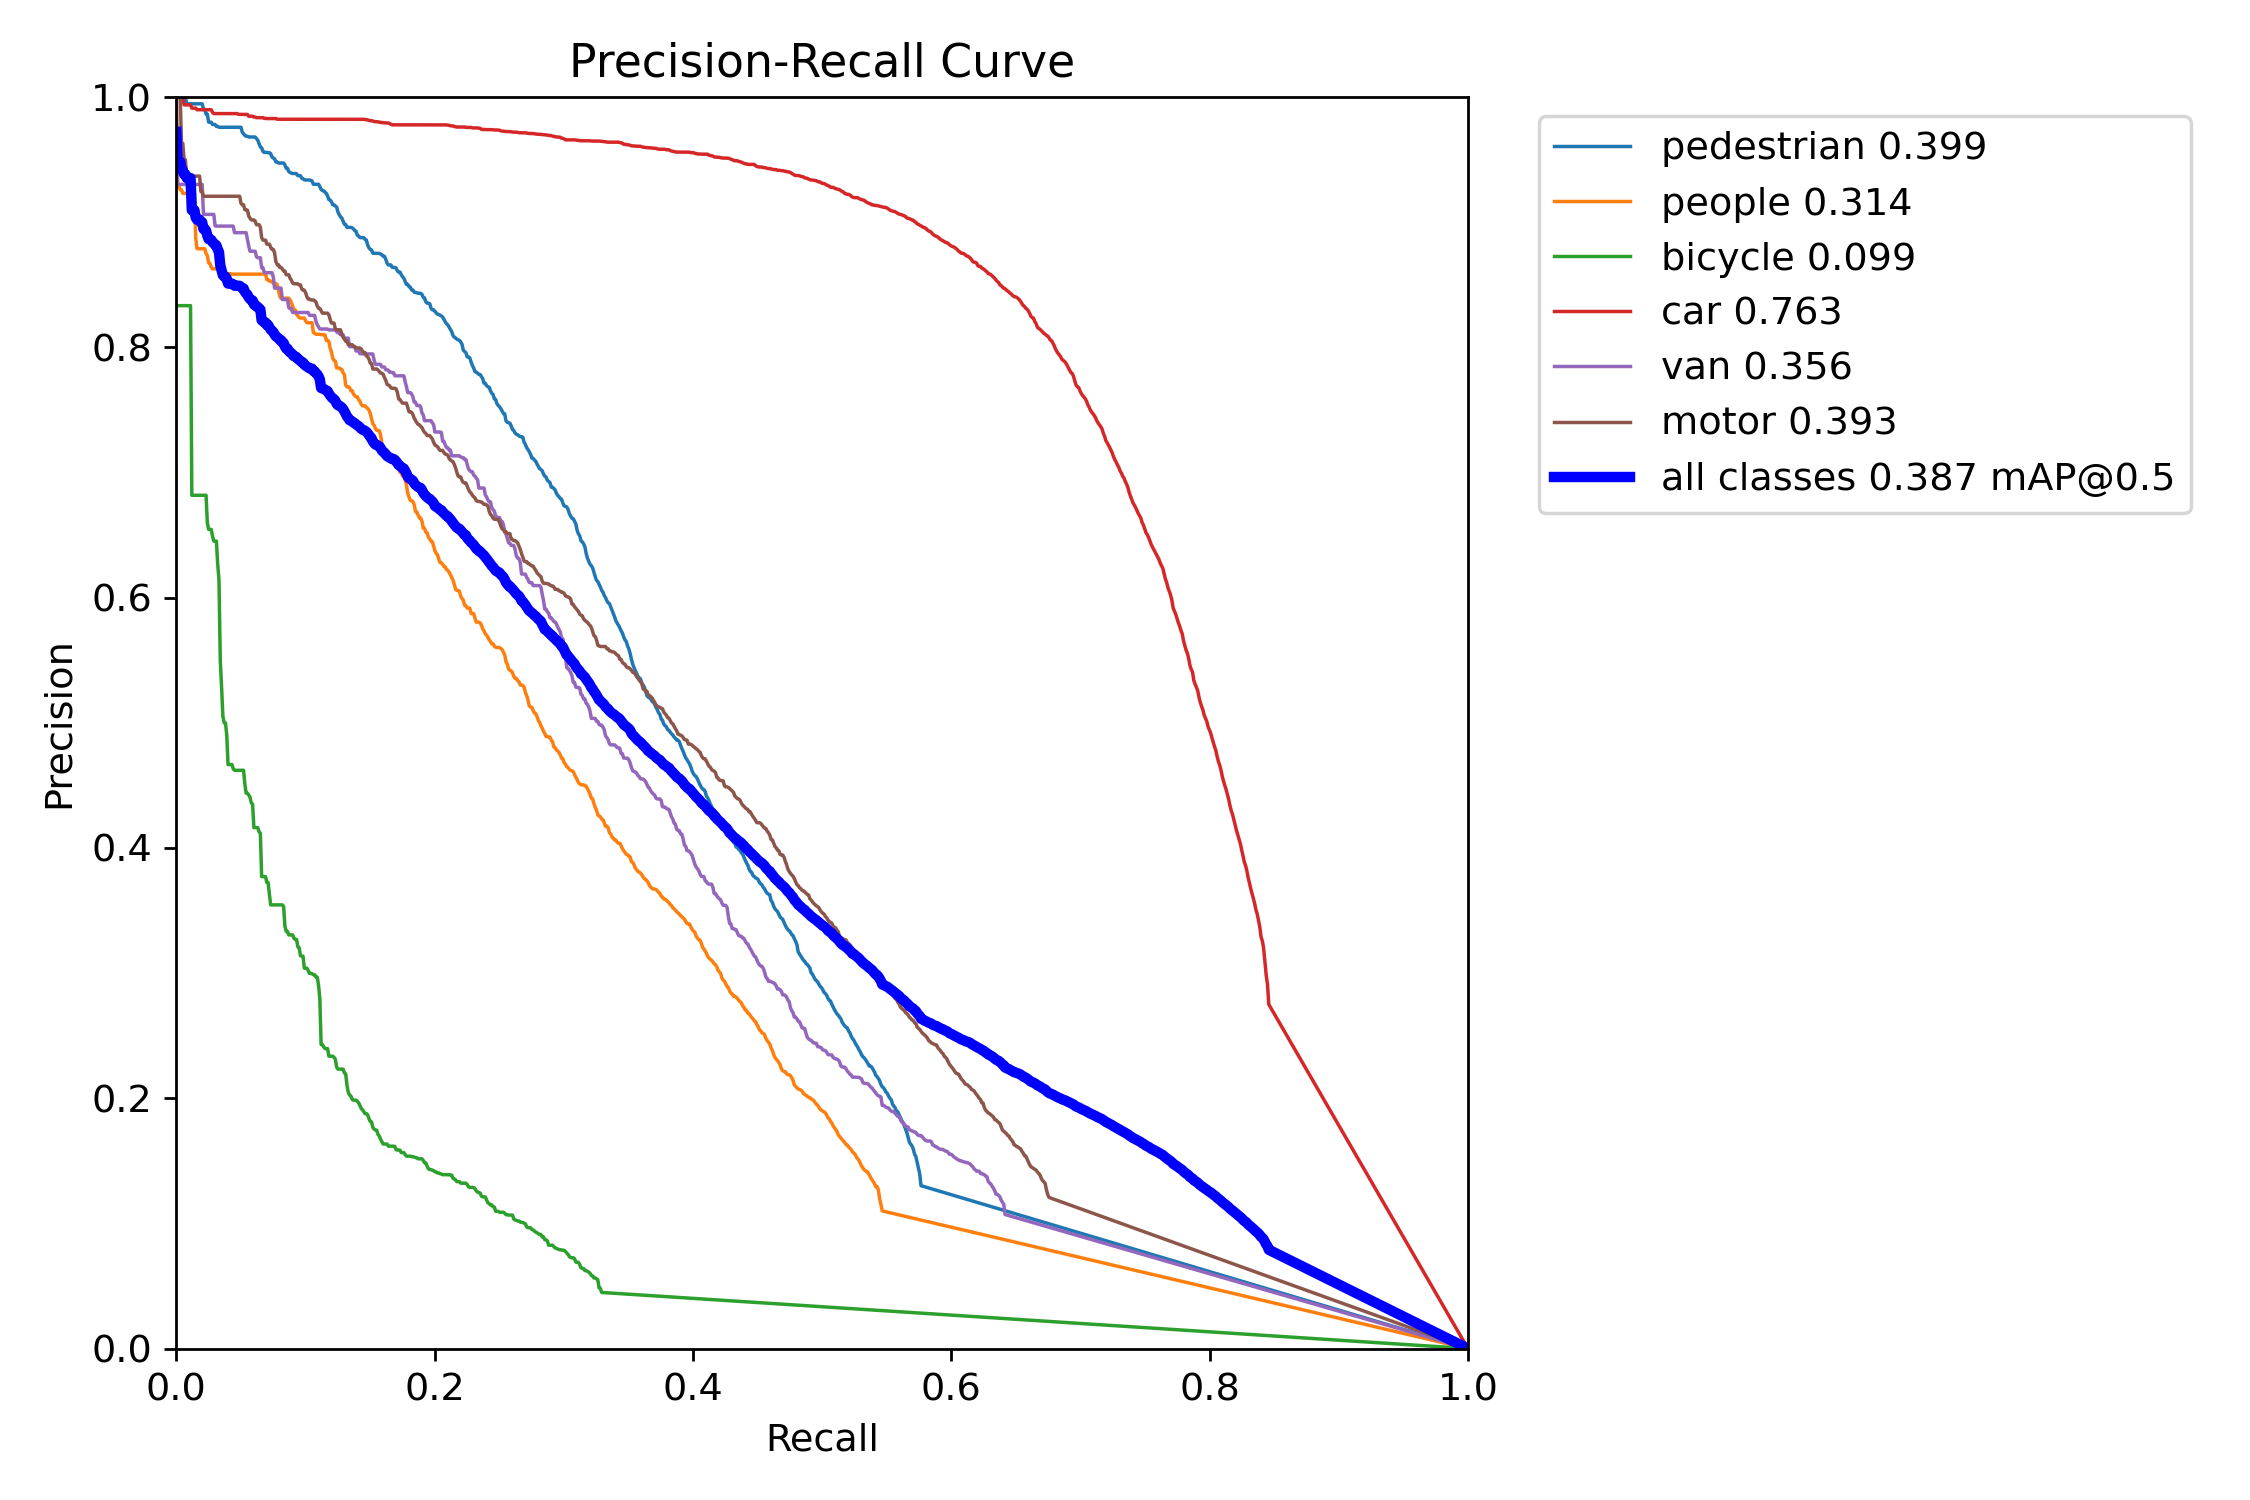
\includegraphics[width=1.0\linewidth]{figs/BoxPR_curve_26n.png}
        \caption{YOLO26n Precision-Recall graph}
        \label{fig:26n}
    \end{minipage}
    \hfill
    \begin{minipage}{0.45\textwidth}
        \centering
        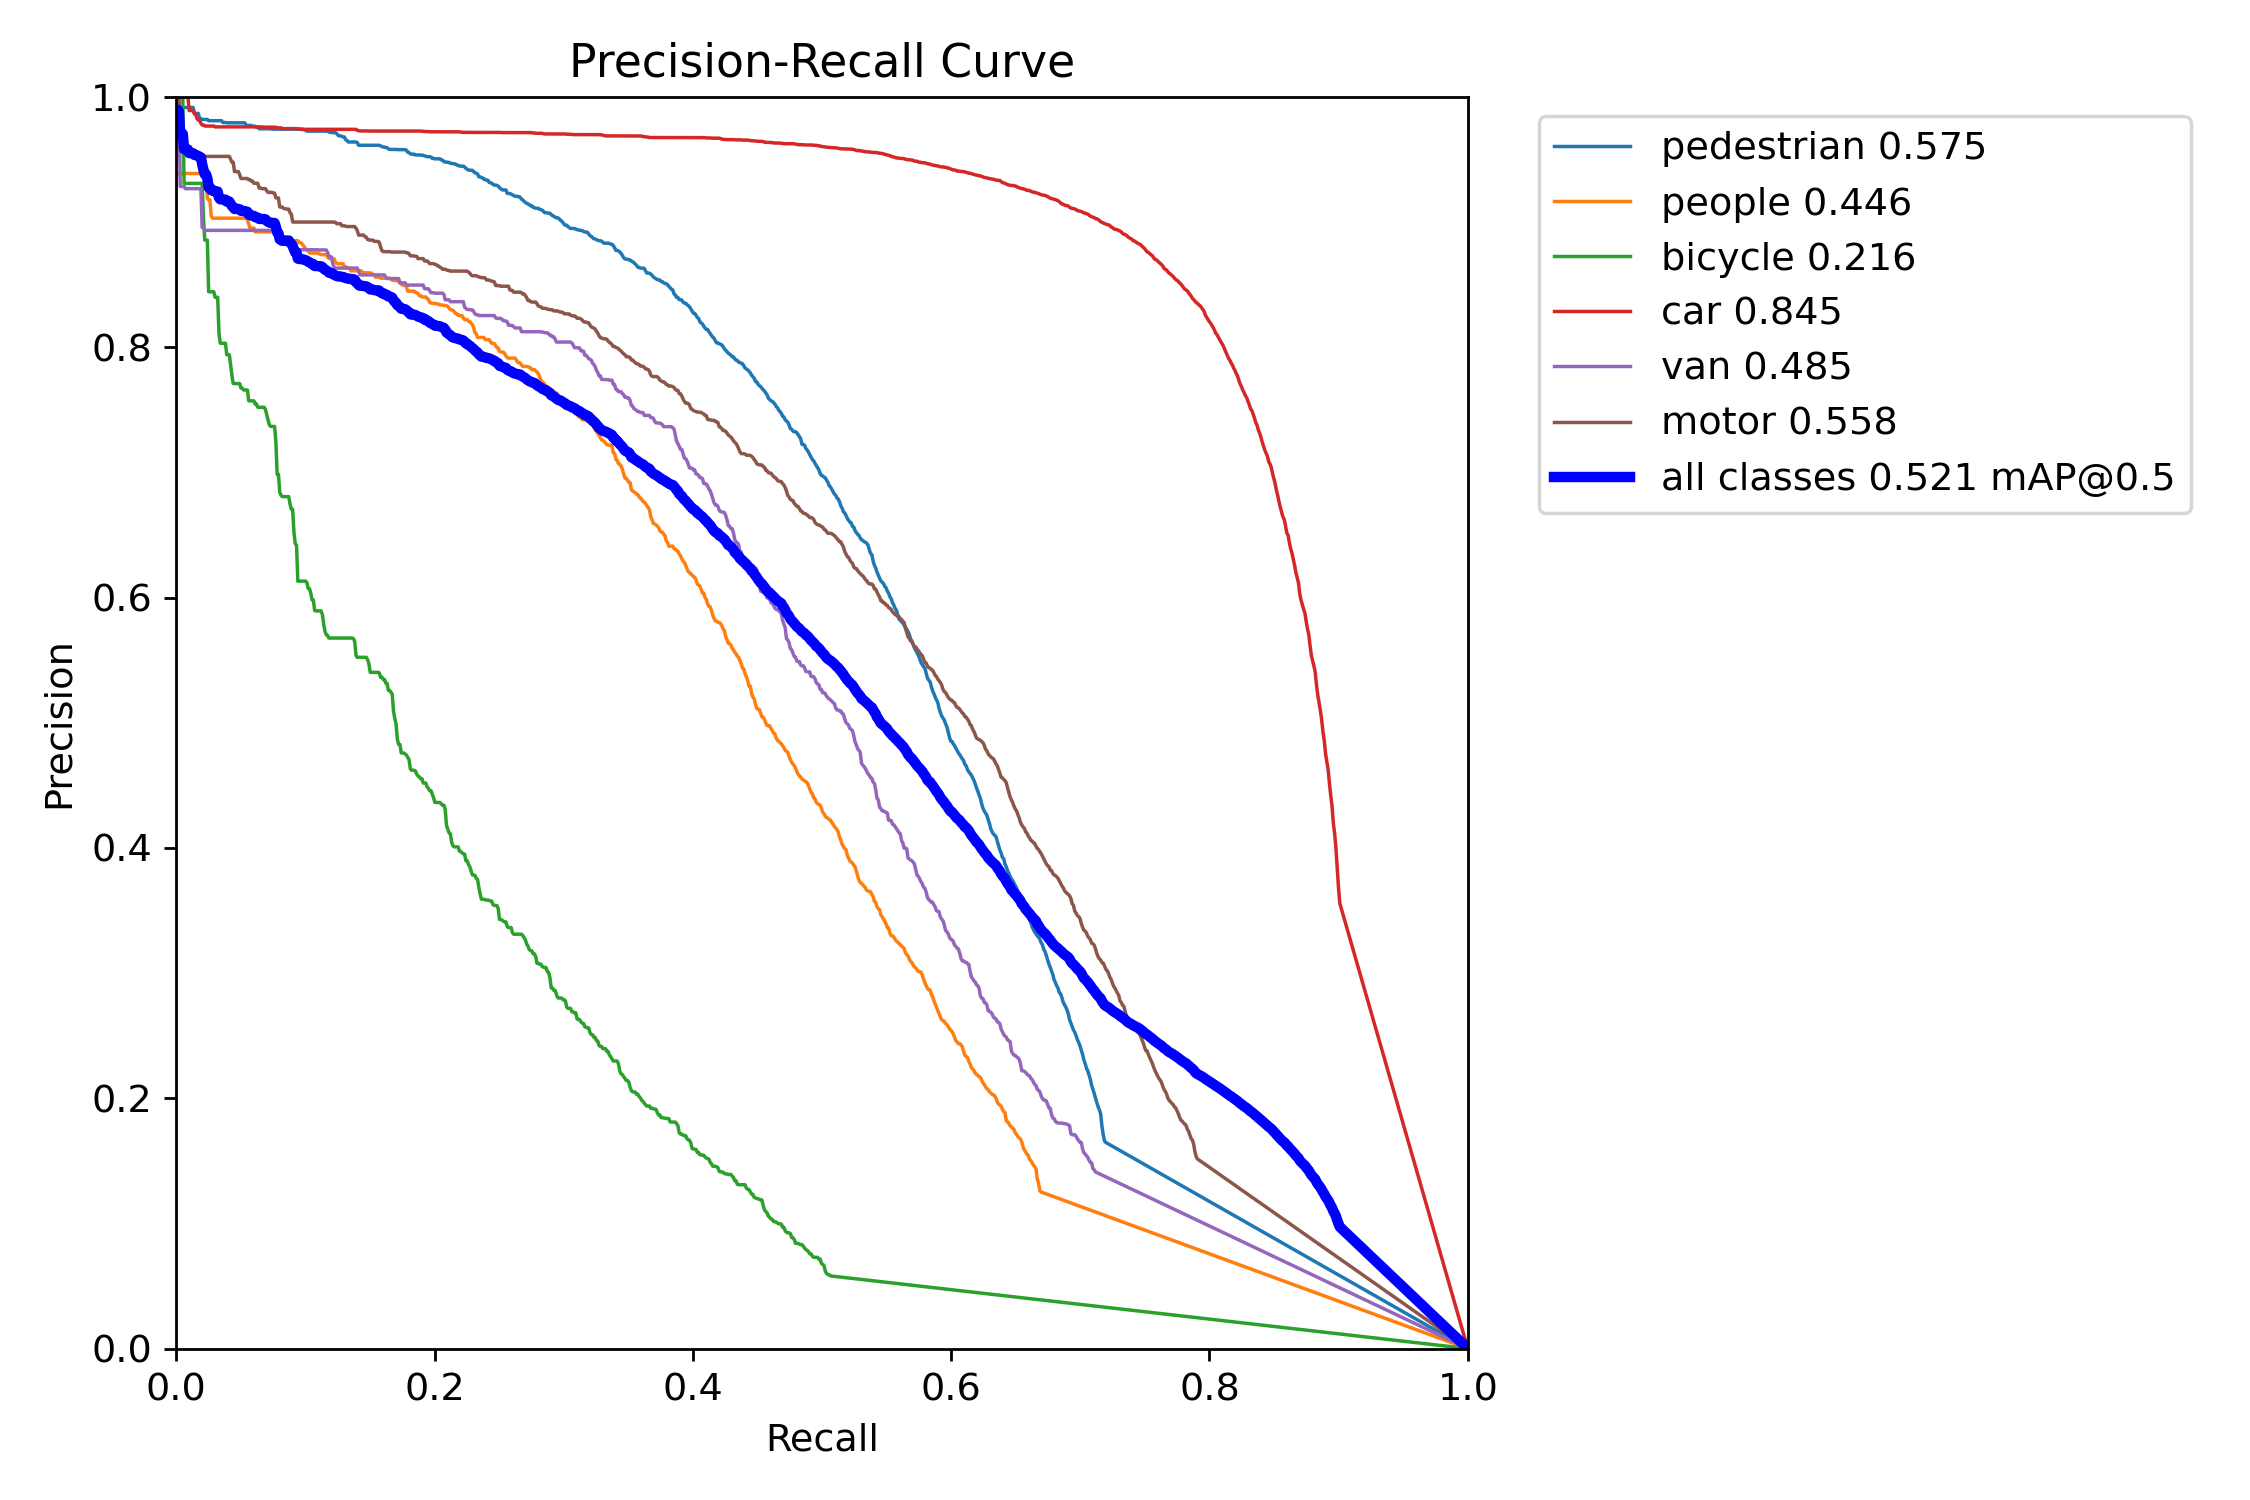
\includegraphics[width=1.0\linewidth]{figs/BoxPR_curve_26l.png}
        \caption{YOLO26l Precision-Recall graph}
        \label{fig:26l}
    \end{minipage}
\end{figure}

The detection results were based on precision and recall. Recall is defined as a measure of whether the 'model has predicted every time it should have'. For the suspect tracking use case, missing a target detection is worse than a False Positive, hence recall is prioritised. Precision is defined by a measure of 'when a model predicts, how often does it predict correctly'. A metric combining precision and recall known as the  'average precision', can be roughly measured by finding the area under the Precision-Recall curves. 

The Precision-Recall curves of the \gls{yolo}v26n and \gls{yolo}v26l are visualised in Figure \ref{fig:26n} and Figure \ref{fig:26l} - as expected the larger \gls{yolo}26l yielded a better average precision as evidenced by the larger area under the curve, with optimal confidence scores of the 26l and 26n at 0.242 and 0.163 respectively - these points were chosen for their maximised  F1 scores \cite{v7labs_map}. 

\subsection{Tracking} \label{tracking}
Tracking allows the drone to aptly identify and differentiate between different objects or suspects between frames, ensuring the drone pursues the same individual suspect. This is done simply by adding a unique ID to each detection. Tracking robustness is especially important when dealing with ego-motion (the movement of the camera itself), in \gls{mot} scenarios such as crowds where it is vital the target is not confused with other civilians, and in target occlusions (suspect goes out of view for a few frames). The next section will discuss the most suitable tracking algorithm for the \gls{pads} use case. 

\subsubsection{Tracking Algorithms}
\textbf{DeepSORT} \quad Historically, DeepSORT \cite{wojke2017simple} served as the industry standard, utilising a deep \gls{reid} network to associate targets based on visual appearance. However, the computational overhead required to extract deep feature embeddings for every detection creates unacceptable latency on constrained edge hardware like the Jetson Orin NX chosen in Section [hardware]. Furthermore, DeepSORT inherently discards low-confidence bounding boxes, leading to track fragmentation when a suspect is temporarily obscured by environmental artifacts.

\textbf{ByteTrack} To address the limitations of confidence thresholding, ByteTrack \cite{zhang2022bytetrack} introduced a novel data association method that retains low-scoring detection boxes, utilising spatial \gls{iou} to maintain tracks during severe occlusions, but completely removed \gls{reid}. While computationally highly efficient, ByteTrack's pure reliance on a spatial distance metrics renders it vulnerable to drone ego-motion; sudden gimbal pans introduce non-linear pixel shifts that the filter misinterprets as target acceleration, resulting in \gls{idsw}.

\textbf{\gls{botsort}} Consequently, \gls{pads} perception architecture implements \gls{botsort} \cite{botsort}. \gls{botsort} inherits the robust low-confidence association matrix of ByteTrack but integrates a critical \gls{cmc} module. By extracting global background keypoints to calculate an affine transformation matrix between frames, \gls{botsort} mathematically isolates the target's true kinematic motion from the drones's ego-motion. This ensures the Kalman filter maintains strict spatial accuracy during aggressive aerial maneuvers, providing an artifact-free trajectory array. \gls{botsort} also improves upon the ByteTrack Kalman filter's 7-dimensional state vector, which estimates an aspect ratio for the bounding box, to an 8-dimensional state vector which explicitly estimates the width and height of the bounding box \cite{botsort}. This allows for tighter bounding box predictions. \gls{botsort} also implements a novel \gls{iou}-\gls{reid} fusion strategy using a gating mechanism - once the \gls{iou} distance meets a set threshold, only then is \gls{reid} similarity considered and fused. 

While ByteTrack offers the lowest computational latency by omitting \gls{reid} and \gls{cmc} \cite{bot_vs_byte_2024}, it is fundamentally incompatible with a highly dynamic drone platform \cite{bytrack_uav_incompatibility}. The marginal speed increase of ByteTrack is entirely negated by its catastrophic failure to handle drone ego-motion. BoT-SORT provides the optimal mathematical compromise \cite{bot_vs_byte_2024}: it is significantly faster than legacy DeepSORT through gated \gls{reid} execution, meaning not all detections are processed through \gls{reid}, yet maintains the strict spatial tracking accuracy required during high-speed aerial maneuvers. Aharon et al. \cite{botsort} compared different tracking algorithms and found \gls{botsort} to perform the most accurately when tested against \gls{mot} benchmark datasets, \textbf{hence confirming \gls{botsort} as the chosen tracker}.  

\subsubsection{BoT-SORT Implementation}\label{botsort yaml}
Implementing \gls{botsort} is done simply by passing a YAML configuration file to the Ultralytics \gls{api}\cite{ultralytics_tracking}. This is done in conjunction with choosing a specific \gls{yolo} detection model to be used with the tracker. Importantly, choice of detection model affects the threshold values to be set in the YAML  configuration file, mainly based on object detection metrics discussed in Section \ref{distributed} and qualitative 'fine-tuning'. 

Within this distributed architecture, the primary function of the high-capacity \gls{yolo}v26l is to compensate for the edge model's limitations, ensuring trajectory continuity by resolving occlusions and mitigating \gls{idsw}. Conversely, the edge-deployed \gls{yolo}v26n is not expected to independently manage these severe edge cases. Instead, its configuration is strictly optimised for target acquisition. In a law enforcement context, suspect omission (False Negatives) represents worse state than suspect hallucination (False Positive); thus, the edge tracker is tuned to heavily prioritise detection recall. Table \ref{tab:yaml_config} details the specific \gls{botsort} hyperparameters selected to enforce these distinct operational roles for the models trained in Section \ref{distributed_training}.


\begin{table}[H]
    \centering
    \begin{tabular}{|c|c|c|}
    \hline
       Parameter  & YOLOv26n & YOLOv26l\\
        \hline
       tracker\_type & bot\_sort & bot\_sort\\
        \hline
       gmc\_method & sparseOptFlow & sparseOptFlow\\
        \hline
       track\_high\_thresh & 0.163 & 0.231\\
        \hline
       new\_track\_thresh & 0.3 & 0.7\\
        \hline
       with\_reid  & True & True\\
        \hline
       track\_buffer & 30 & 60\\
    \hline
    \end{tabular}
    \caption{\gls{botsort} YAML configuration parameters}
    \label{tab:yaml_config}
\end{table}

\textbf{Hyperparameter details} Selecting \gls{botsort} as a tracker and turning on \gls{cmc} was done by setting \texttt{tracker\_type} and \texttt{gmc\_methods}. \texttt{track\_high\_thresh} is the first stage confidence threshold to continue tracking an object, and  was set by matching with each model's respective F1 score \cite{ultralytics_tracking}. \texttt{new\_track\_thresh} represents the ease with which the system begins a new track, with a higher value being more strict. This is where the edge model prioritises tracking recall by setting a lower value at 0.3, and the \gls{cgs} model prioritises track precision by setting a larger value of 0.7. \texttt{track\_buffer} was set to 60 frames for the central model so that a lost ID would be held in memory for enough time (3 seconds at 20 \gls{fps}) to allow for medium-long occlusions, with occlusion handling being less important in the edge case. \texttt{with\_reid} was set to True on both to facilitate track recovery, despite the computational overhead \cite{bot_vs_byte_2024}. 

\subsubsection{Tracking Occlusion Handling Evaluation}
The tracking architecture must be able to handle partial and full obstructions of the target, also known as \textbf{occlusions}. The most extreme example is temporary complete occlusion, whereby the target disappears completely from view before re-emerging, which will be considered here. It can be inferred that if the system can resolve this extreme edge case, lesser partial occlusions can also be handled. The architecture was tested against several occlusion sequences from the UAV123 dataset \cite{mueller2016benchmark}, most of which contained sub-3-second occlusions. An example is shown in Figure \ref{fig:occlusion_handling}. 

\begin{figure}[H]
    \centering
    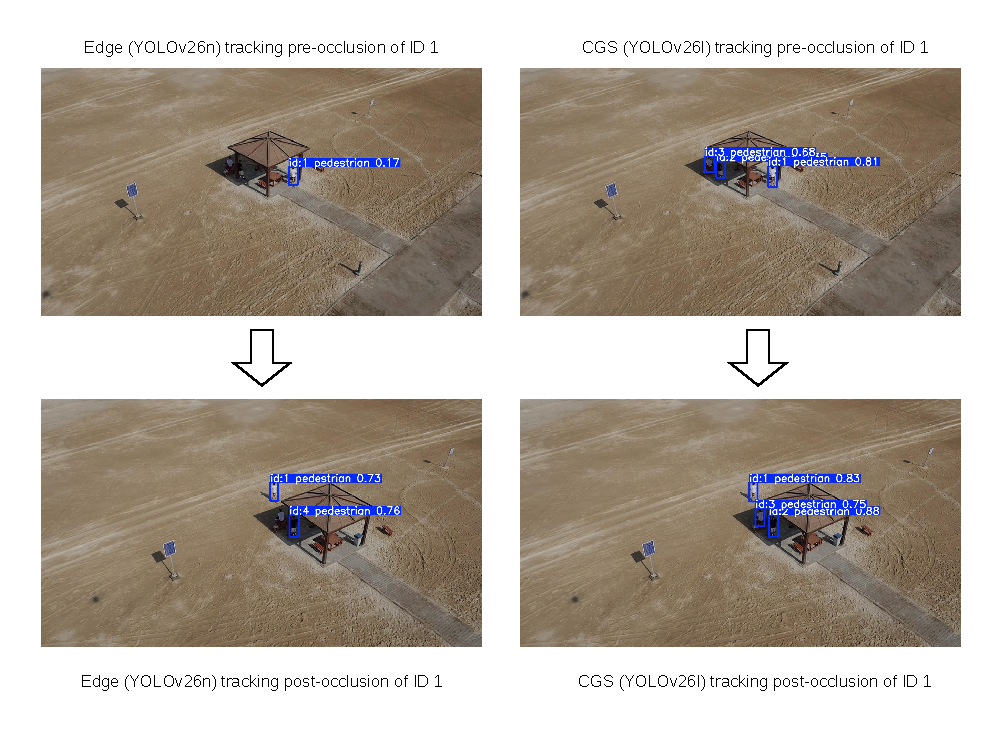
\includegraphics[width=1\linewidth]{figs/occlusion_example.pdf}
    \caption{Occlusion Handling onboard (left) and centrally (right)}
    \label{fig:occlusion_handling}
\end{figure}

The edge system was able to correctly reidentify ID: 1  post-occlusion, a result of the \gls{botsort} Kalman filter accurately predicting the target's linear kinematic trajectory during the brief obstruction. However, it does completely miss detections of a secondary pedestrian in both frames (False Negatives), and incurs multiple \glspl{idsw}, erroneously spawning a fourth track (ID: 4) in a sequence of only 3 objects. Figure \ref{fig:occlusion_handling} also displays a markedly large disparity in detection certainty, with a 4.76 times increase in the pre-occlusion edge system ID: 1 confidence (0.17) compared to the \gls{cgs}'s (0.81). This comes from the  edge model's lower recall (as evidenced in Section \ref{distributed}), which leads to the demonstrated increase in missed detections and track fragmentation. On the other hand, the \gls{cgs} accurately maintains track of all three IDs in Figure \ref{fig:occlusion_handling}, handling ID 1's occlusion and incurring no \glspl{idsw}, validating the \gls{cgs}'s superior tracking performance and hence its operational necessity for reliable tracking persistence.  

\subsubsection{Multiple Object Tracking Evaluation}
It is vital the tracking architecture is able to accurately track in \gls{mot} scenarios. Mitigating \glspl{idsw} or losing track of a suspect evading pursuit by entering dense object sceneries such as crowds is important in a populated London use case. Hence, this section will attempt to measure the overall system's \gls{mot} tracking accuracy. 

Despite it proving to be notoriously difficult to measure, there are several metrics for measuring the ability of a tracker to track multiple targets, but they can largely be categorised into metrics which prioritise \gls{assoca} and \gls{deta}. \gls{assoca} measures the ability of a tracker to link detections over time to the same ID, and \gls{deta} measures the alignment of a tracker between the set of all predicted detections and the set of all ground-truth detections \cite{mendez2024motmetrics}. The main two metrics which will be considered are the \gls{mota} and IDF1, the former priotising \gls{deta} and the latter \gls{assoca} \cite{mendez2024motmetrics}. Despite it being the current industry standard, measuring \gls{hota} has been omitted as it provides a 'middle-ground' metric between \gls{mota} and IDF1 \cite{Luiten_2020}, which proves to be redundant in the \gls{pads} use case. This is because as mentioned in Section \ref{botsort yaml}, the \gls{cgs} tracking exists to prioritise smooth tracks and minimise \gls{idsw}, which is adequately measured by IDF1, and the edge model's aim is to prioritise detection recall, as measured by \gls{mota}. Hence, \gls{hota} is not needed.

\textbf{\gls{mota}} counts False Negatives \(FN\) and  False Positives \(FP\) at every frame index \(t\) and Identity Switches \(IDSW\), which occur when a single \gls{gt} assignment is assigned to different assignments over time. 

\begin{equation}
  MOTA=1-\frac{∑_t(FN_t+FP_t+IDSW_t )}{∑_tGT_t}
  \label{eq:mota}
\end{equation}

\textbf{IDF1} addresses some of MOTA’s limitations by focusing on how long the tracker correctly identifies an object, rather than just counting errors. It’s based on the concept of Identification Precision (IDP) and Identification Recall (IDR).

\begin{equation}
  IDF1=  \frac{2×IDTP}{2×IDTP+IDFP+IDFN}
  \label{eq:idf1}
\end{equation}

Where, IDTP (ID True Positive) is the number of correctly identified detections,
IDFP (ID False Positive) is the tracker predictions that don’t match any ground truth, and IDFN (ID False Negative) are \gls{gt} trajectories that failed to track.

 The configured edge and \gls{cgs} trackers from Section \ref{botsort yaml} were evaluated against a labelled sequence from the \gls{mot} benchmark dataset from VisDrone2019-MOT \cite{visdrone2019-MOT}. A particularly complex sequence from crowded scenery was chosen to test the tracking architecture's edge case, as illustrated in Figure \ref{fig:crowd}.

\begin{figure}[H]
     \centering
     
     % --- LEFT IMAGE ---
     \begin{subfigure}[b]{0.49\textwidth}
         \centering
         
         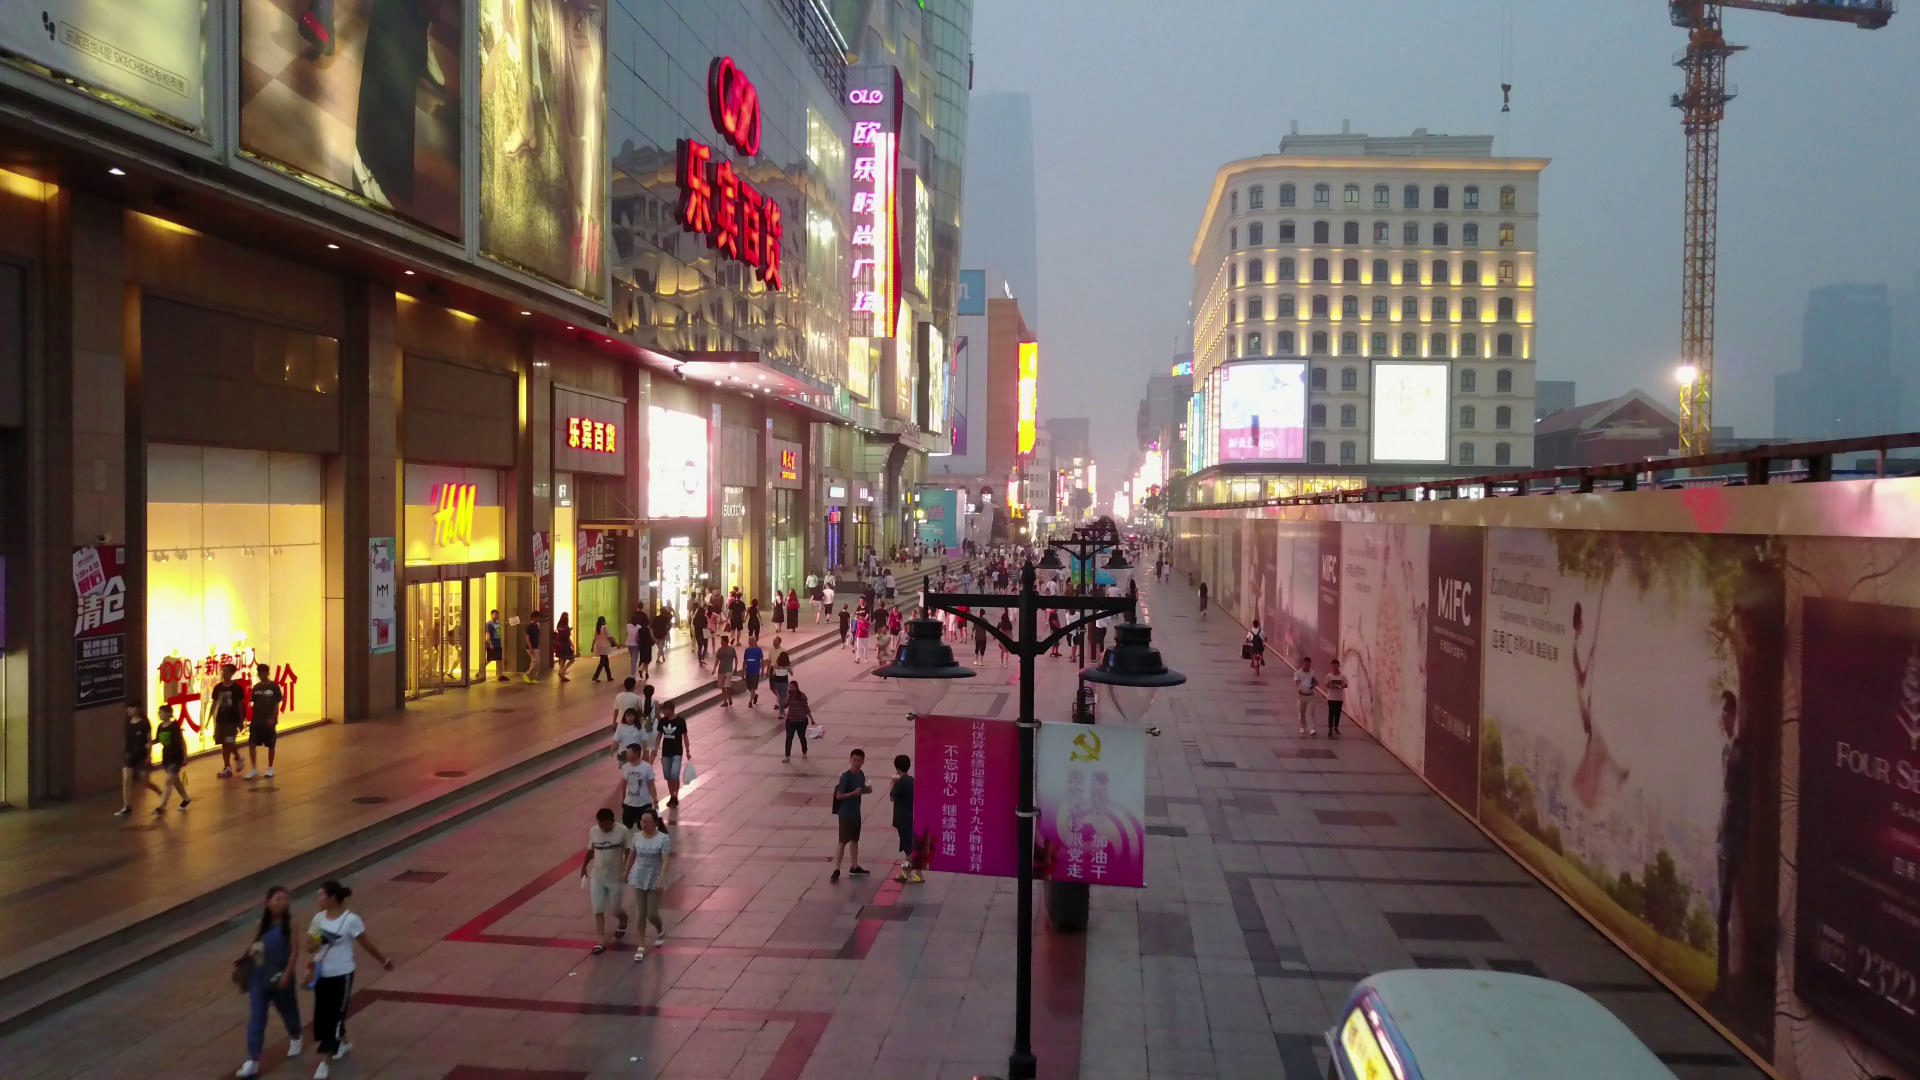
\includegraphics[width=\linewidth]{figs/visdrone_mot_crowd.jpg}
         \caption{VisDrone2019-MOT test sequence example image}
         \label{fig:crowd}
     \end{subfigure}
     \hfill % Add horizontal space between the images
     % --- RIGHT IMAGE---
     \begin{subfigure}[b]{0.49\textwidth}
         \centering
         
         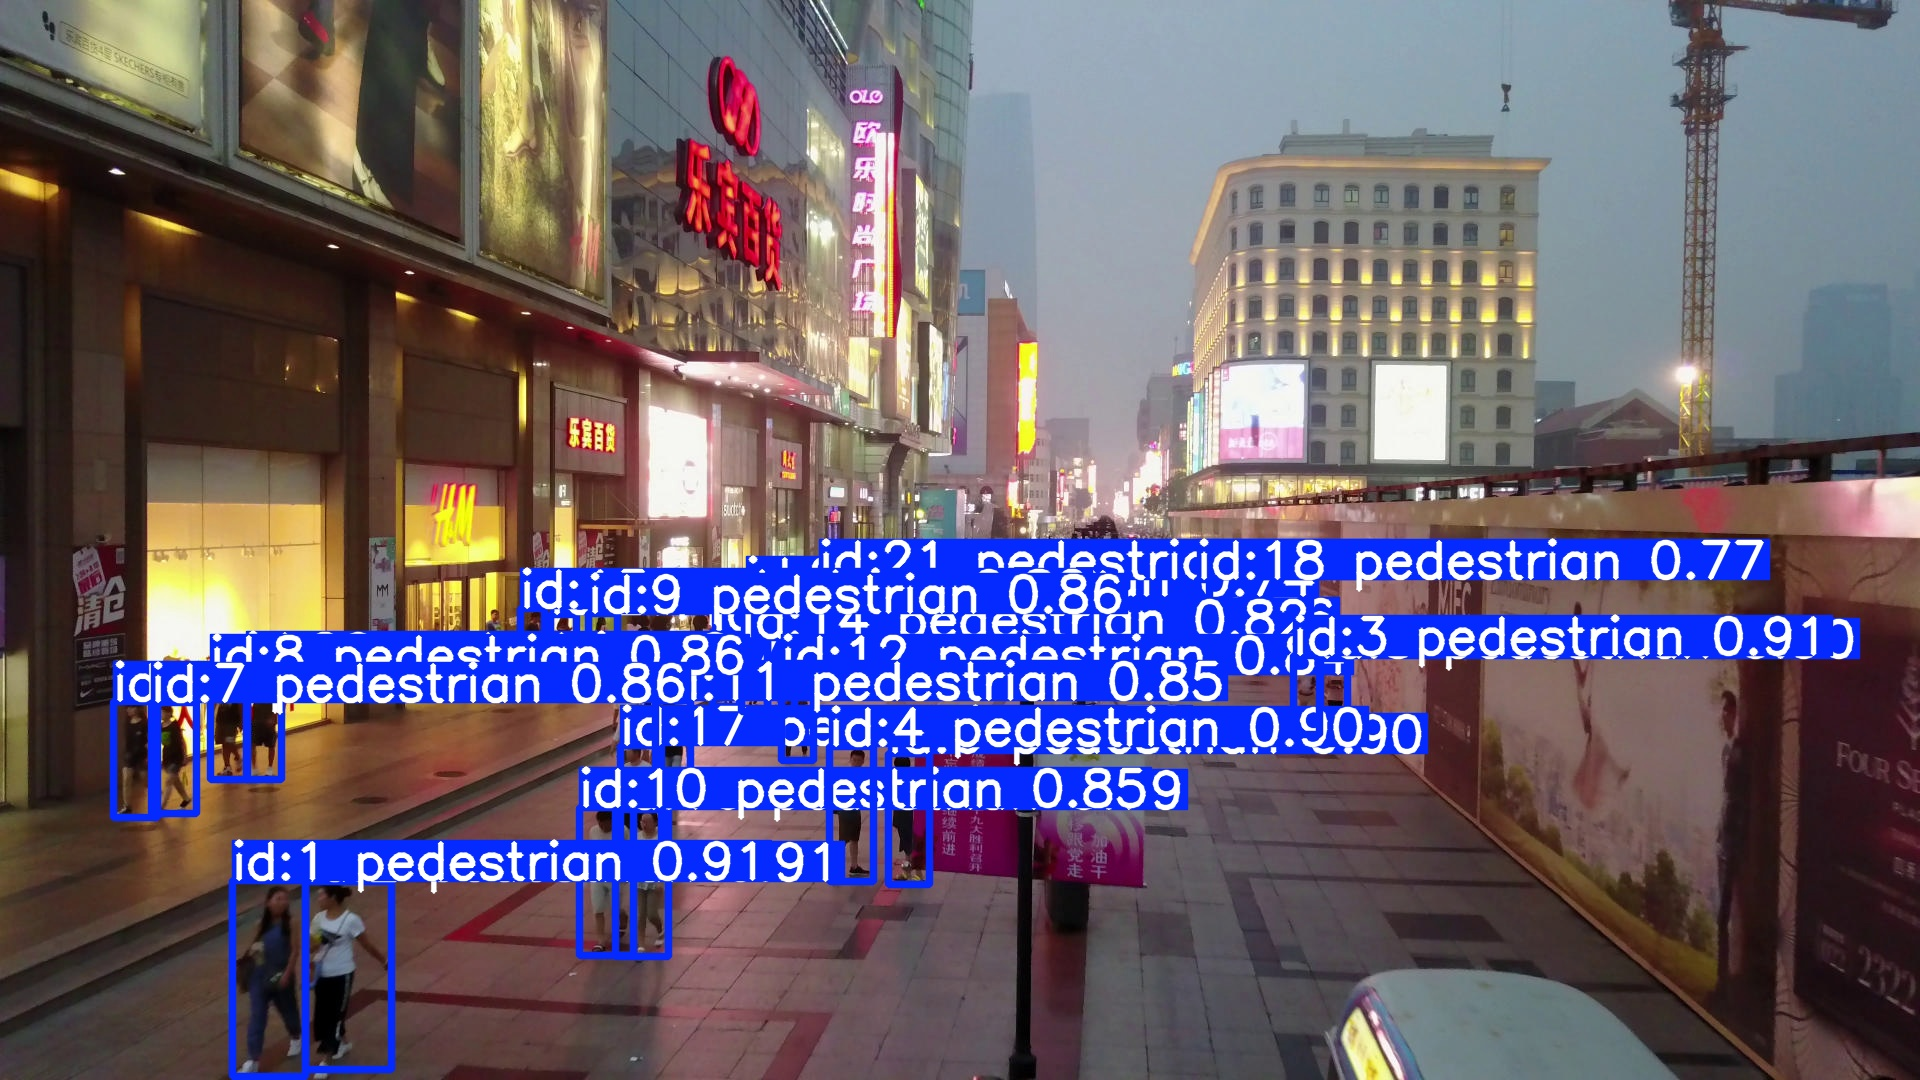
\includegraphics[width=\linewidth]{figs/visdrone_mot_crowd_tracked.jpg}
         \caption{After \gls{cgs} Tracking}
         \label{fig:crowd_tracked}
     \end{subfigure}
     
     % --- MAIN CAPTION ---
     \caption{A visual before-and-after comparison of detection and tracking performance in high-density crowded scenery using the \gls{cgs} tracking architecture.}
     \label{fig:crowds_comparison}
 \end{figure}

The final evaluation metrics are displayed in Figure \ref{fig:tracking_bar_charts}.

\begin{figure}[H]
    \centering
    
    % --- CHART 1: ACCURACY (MOTA & IDF1) ---
    \begin{minipage}{0.48\textwidth}
        \centering
        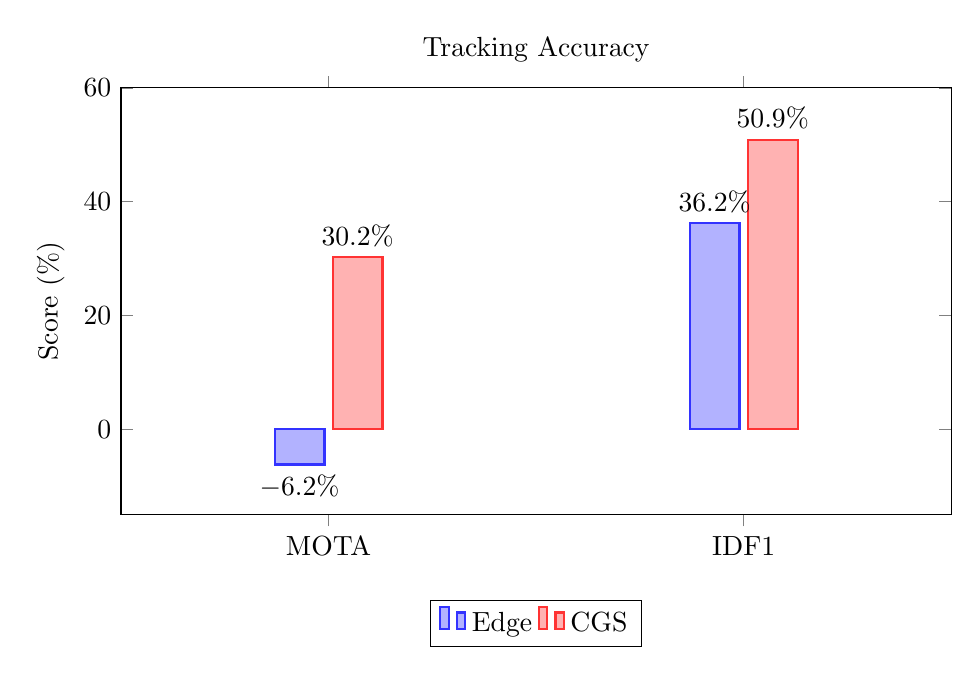
\begin{tikzpicture}
            \begin{axis}[
                ybar=3pt, % Spacing between bars
                bar width=18pt,
                width=\textwidth,
                height=7cm,
                enlarge x limits=0.5,
                ymin=-15, ymax=60,
                ylabel={Score (\%)},
                symbolic x coords={MOTA, IDF1},
                xtick=data,
                nodes near coords={\pgfmathprintnumber\pgfplotspointmeta\%},
                nodes near coords align={vertical},
                legend style={at={(0.5,-0.2)}, anchor=north, legend columns=-1},
                title={Tracking Accuracy}
            ]
            % Edge Model Data
            \addplot[fill=blue!30, draw=blue!80, thick] coordinates {(MOTA,-6.2) (IDF1,36.2)};
            % CGS Model Data
            \addplot[fill=red!30, draw=red!80, thick] coordinates {(MOTA,30.2) (IDF1,50.9)};
            
            \legend{Edge, CGS}
            \end{axis}
        \end{tikzpicture}
    \end{minipage}\hfill
    % --- CHART 2: ERRORS (IDSW) ---
    \begin{minipage}{0.48\textwidth}
        \centering
        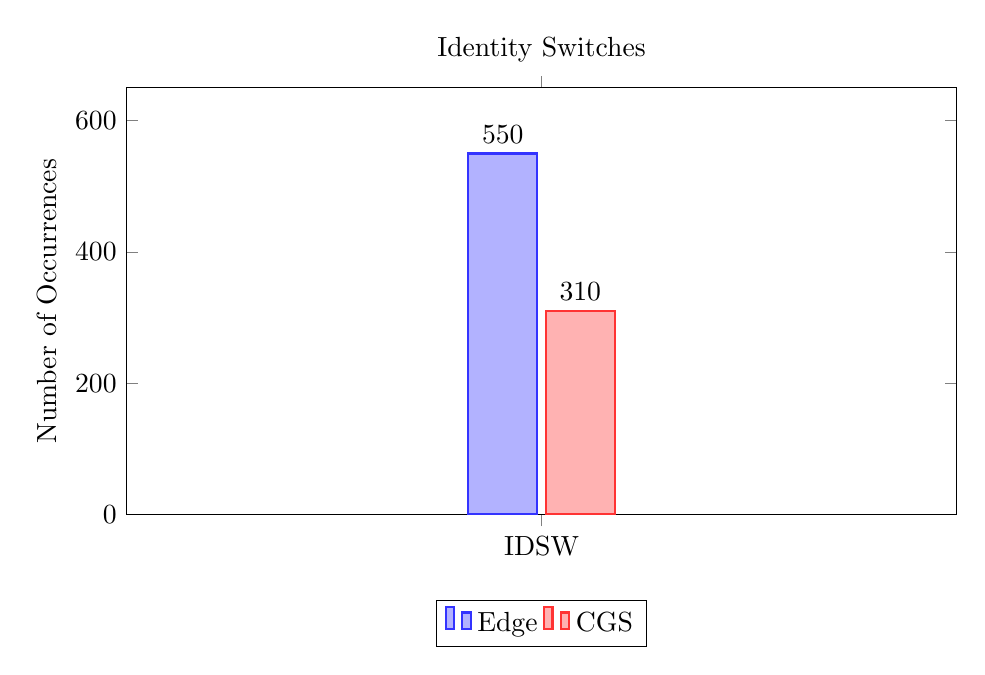
\begin{tikzpicture}
            \begin{axis}[
                ybar=3pt,
                bar width=25pt,
                width=\textwidth,
                height=7cm,
                enlarge x limits=0.5,
                ymin=0, ymax=650,
                ylabel={Number of Occurrences},
                symbolic x coords={IDSW},
                xtick=data,
                nodes near coords,
                nodes near coords align={vertical},
                legend style={at={(0.5,-0.2)}, anchor=north, legend columns=-1},
                title={Identity Switches}
            ]
            % Edge Model Data
            \addplot[fill=blue!30, draw=blue!80, thick] coordinates {(IDSW,550)};
            % CGS Model Data
            \addplot[fill=red!30, draw=red!80, thick] coordinates {(IDSW,310)};
            
            \legend{Edge, CGS}
            \end{axis}
        \end{tikzpicture}
    \end{minipage}
    
    \vspace{0.25cm} % Add some breathing room below the charts
    \caption{Comparative tracking performance between the Edge (YOLOv26n) and CGS (YOLOv26l) tiers.}
    \label{fig:tracking_bar_charts}
\end{figure}

The need for a \gls{cgs} is made immediately obvious by the 36.4 percentage points recovery in \gls{mota} score from the negative one recorded by the edge tracker. This is a direct consequence of a higher number of FNs, FPs and \glspl{idsw} being recorded from the lower complexity \gls{yolo}v26n, resulting in a top-heavy negative fraction in Equation \ref{eq:mota}. As expected, the \gls{cgs} also provided smoother, less fragmented tracking evidenced by the 14.7 percentage points superior IDF1 score and 240 fewer \glspl{idsw} over the test sequence's 328 frames. The edge model averaged a 10.4ms inference time compared to 15.3ms with the \gls{cgs} when ran on Kaggle's Tesla 2 x T4 \glspl{gpu}, highlighting the edge model's strength with faster speeds, which is exacerbated with the \gls{cgs}'s communication delay. Overall, lower \gls{mota} and IDF1 scores and high \gls{idsw} scores present the system's difficulty in dealing with highly packed crowds, although decent tracking perception is still present. This highlights the importance of an operator to continually guide the drone towards obstructed target. 

\subsection{Central Ground Server}
The need for a \gls{cgs} for cloud perception is evidenced in Section \ref{distributed}. The edge detection model (YOLOv26n) struggled with lost tracks when handling occlusions and dense multi-object tracking scenarios, and is generally more prone to missed and false detections. This is primarily due to the lower complexity of the YOLO26vn, which the edge system is restricted to due to strict power consumption constraints on the drone \textbf{[Hardware]}. These same constraints do not apply to the \gls{cgs}, which has a virtually unlimited power budget and  the ability to use more powerful compute hardware, in this case the RTX 4090. Ntousis et al. \cite{ntousis} found that when testing an edge model in isolation, nearly a third of all targets were lost, whereas integrating a \gls{cgs} allowed for 70\% of these lost tracks to be recovered. 

For the server to be able to provide timely corrections despite the 150ms \gls{rtt} between the \gls{cgs} and the drone discussed in [Hardware], Ntousis et al. \cite{ntousis} suggests sending \textit{'a sequence of timestamped predictions, from which the} [drone] \textit{selects the closest to its current time'}. This suggests a proactive approach; however, several other methods also exist for handling this latency, as discussed in the following Section \ref{cloud based perception}. 

\subsubsection{Cloud-based perception} \label{cloud based perception}
The following paragraphs discuss different currently-used methods for cloud perception when dealing with dealing with latency. 

\textbf{\gls{oosm}} \gls{oosm} is a traditional retroactive approach to latency compensation, often implemented via retrodiction using Linear Kalman Filters \cite{bar_shalom}. Rooted in standard control theory, \glspl{oosm} handles the 150ms delay by maintaining a state vector and retroactively integrating the server's delayed measurements into the drone's current timeline. However, this method presents two major limitations for drone edge deployment. First, it fundamentally assumes linear flight pathways, making it ill-equipped to model non-linear spatial fluctuations typical of drone trajectories. Secondly, Shi et al. \cite{shimodified2020} demonstrates that high time complexity arising from retrodiction introduces a severe computational overhead that is prohibitively expensive for resource-constrained edge hardware, hence making it unsuitable for the \gls{pads} perceptive framework.

\textbf{Mamba \gls{ssm}} In contrast to retroactive filters, modern \glspl{ssm} such as Mamba offer a proactive, deep-learning-based alternative for future prediction. Mamba is highly adept at modeling complex, non-linear pathways and operates with a linear time complexity that scales exceptionally well for sequence modeling. It is specifically designed to capture long-term dependencies and global temporal dynamics \cite{gu2024mambalineartimesequencemodeling}. However, Mamba relies on massive context windows—often requiring tens of thousands of frames—to build effective internal state representations. As noted in recent literature, \glspl{ssm} lack 'explicit mechanisms to model fine-grained spatial interactions and local motion patterns, resulting in suboptimal performance for representing short-term spatial–temporal features' \cite{ZHANG2025130464}. This, coupled with the drone's limited onboard resources, renders the edge system incapable of using such a complex model. 

\textbf{Predictive compensation} Predictive compensation utilises deep learning to offer a highly effective, proactive solution. These models provide a way to predict short-term dynamics and fine grained spatial fluctuations \cite{ZHANG2025130464}\cite{dong2023tcn}, whilst maintaining low computational overhead required for drone edge deployment. For these reasons, alongside lower memory footprints, predictive compensation was chosen as a method for cloud perception. Final implementation of predictive compensation is discussed in Section \ref{final_data_pipeline}. While numerous sequence-modeling architectures exist for this task, this paper will mainly consider the industry-standard \gls{lstm} model against the highly parallelisable \gls{tcn} architecture, as discussed in Section \ref{sequence_forecasting}. 

\subsection{Comparison of temporal sequence forecasting architectures} \label{sequence_forecasting}
The following few sections will evaluate two different methods of implementing sequence forecasting, namely via \glspl{lstm} and \glspl{tcn}, to determine the best method of implementing predictive compensation. 

\subsubsection{Long Short-Term Memory Model Design}
LSTMs are the industry standard method of path prediction. Ntousis et al. \cite{ntousis} utilised LSTMs as a way to combine the detection models ran onboard and on the CGS, using them ‘to achieve the above combination in the case of communication delays’. LSTMs are a specialised type of \gls{rnn} that utilise a system of gating mechanisms — specifically forget, input, and output gates — to to consider both long- and short-term dependencies between the elements of their input sequences.

However, because \glspl{lstm} process data chronologically, computing the current hidden state (\(h_t\)) strictly requires the output of the previous time step (\(h_{t-1}\)). This inherent sequential dependency renders \glspl{lstm} entirely non-parallelisable. Furthermore, the complex matrix multiplications required within the four internal gating layers significantly increase computational overhead, creating a latency bottleneck when processing high-frequency video data or attempting to retain context over extended temporal sequences \cite{bai2018empirical}. 

Beyond computational inefficiency, the \gls{lstm} architecture exhibits severe vulnerabilities when handling real-world tracking occlusions. Specifically, the forget gate mechanism is highly susceptible to premature state flushing when confronted with sudden input perturbations. If the tracking pipeline experiences a momentary dropout—such as a target passing behind an obstacle—the network may interpret the sudden shift in the input vector as a sequence termination signal. This triggers the forget gate to erroneously discard the accumulated cell state (\(C_{t-1}\)), wiping the historical kinematic context. Consequently, this catastrophic loss of temporal memory severely degrades the \gls{lstm}'s ability to accurately extrapolate the suspect's trajectory upon re-acquisition \cite{milan2016}.

\textbf{\gls{lstm} Design} \quad Using a similar \gls{lstm} structure to the model used in Ntousis et al. \cite{ntousis}, a 64 hidden unit \gls{lstm}, followed by a fully connected layer with linear activation functions was chosen. The \gls{lstm} will look back \textbf{10 frames} into the past, to balance model accuracy with speed and model size. PyTorch’s \gls{lstm} class was utilised to efficiently implement this architecture. \textbf{input -> LSTM -> output diagram?}

\subsubsection{Temporal Convolutional Network Design}

\glspl{tcn} perform series forecasting using dilated causal 1D convolution. While traditional \glspl{cnn} utilise normal convolution, \glspl{tcn} shift the kernel so that they only see [\(t-(k-1),t-(k-2),..,t\)] steps at a time, applying left-padding, if necessary, where k is the kernel length \cite{tcn_medium}. Properties of \glspl{tcn} include: 

\textbf{Dilation} \quad  Depending on the layer, \glspl{tcn} will ‘skip’ neurons, which will allow the model to grow their receptive field (look further into the past) with each layer – this is called dilation. Traditional \glspl{cnn}’ layers grow linearly with increasing receptive field, which leads to inefficient memory usage – \glspl{tcn} allow for large receptive fields without blowing up their memory footprint. Larger receptive field allows for more accurate measurements. Dilation usually increasing exponentially every layer, as shown below.

\textbf{Parallelisation} \quad \glspl{tcn} utilise convolution, which means they can be easily parallelised on a GPU – this allows for faster computation. Whereas \glspl{rnn} such as an \gls{lstm} can only be calculated sequentially since computing the current state requires the previous state.

\textbf{Residual blocks} \quad form the subunits in a \gls{tcn} and usually consist of around 2 convolution layers of the same dilation per block. Each layer is succeeded with a weight normalisation, RelU activation to introduce non-linearities, and then dropout to reduce overfitting and boost computing speed. There is also a residual connection (skip connection) to help reduce the vanishing gradient problem and prevent loss of important signals. Residual blocks are attached sequentially with increasing dilations as in Figure \ref{tcn}. 

\begin{figure}
    \centering
    
\includegraphics[width=1\linewidth]{residual_head.png}
    \caption{TCN Architecture with increasing dilations d at each layer k (1,2,4,8,etc.) \cite{ntousis}}
    \label{fig:tcn}
\end{figure}



\textbf{TCN Design} \quad The TCN will aim for a receptive field of 30 frames, to take advantage of its efficient computation. Based off a similar design to Dong et al. \cite{dong2023tcn}, which used also utilised TCNs for an aerial application, the model will utilise residual heads with 2 convolutional layers. Using the formula for receptive field and assuming the kernel size is three to allow for non-linear pathway prediction:  


\[R=1+2(k-1) \Sigma_{i=0}^{f-1}d_i 
\]
Where \(f\) is the number of residual heads, \(d\) is the exponentially increasing dilation (1, 2, 4 ,8 ,etc.) and 2 arises from there being 2 layers per residual head. Aiming for \(R \approx 30\) frames, and trialing an increasing number of heads:


\begin{table}[H]
    \centering
    \begin{tabular}{|c|c|c|}
    \hline
        Residual heads (\(f\)) & Receptive field (\(R\)) \\
        \hline
        1 & \(R=1+2(3-1)(1)=5\)  \\
        \hline
        2 & \(R=1+2(3-1)(1+2)=13\)  \\
        \hline
        3 & \(R=1+2(3-1)(1+2+4)=29\) \\
        \hline
    \end{tabular}
    \caption{Different receptive fields with varying \(f\)}
    \label{tab:receptive_field_calc}
\end{table}


Hence, the final chosen model used \textbf{3 residual heads each with 2 convolution layers}. \textbf{TCN Diagram?}

\subsubsection{Training}
Both models were trained using the \textbf{Adam optimiser} for its ability to handle sparse gradients and noisy data by adapting learning rates for individual parameters. To ensure a fair comparison between the models, a base learning rate of 0.001 was used in both cases. Both models were trained over 100 epochs with a batch size of 64, on Kaggle using dual Tesla T4 \glspl{gpu}. The VisDroneVDT-2019 \cite{visdrone2019} dataset was used for training.

\begin{figure}[H]
    \centering
    \begin{tikzpicture}
        \begin{axis}[
            width=0.8\textwidth,
            height=6.5cm,
            xlabel={Epoch},
            ylabel={\gls{mse} Loss},
            legend style={font=\tiny},
            legend pos=north east,
            grid=major,
            grid style={dashed, gray!30},
            xmin=0, xmax=100,
            % We can set a log scale for the Y axis to better see the changes
            ymode=log,
            log basis y={10}
        ]
        
       % 1. TCN Validation (Solid Blue)
        \addplot[color=blue, thick, solid] 
            table [col sep=comma, x=Epoch, y=ValLoss] {logs/tcn_training.csv};
        \addlegendentry{TCN Validation}

        % 2. TCN Training (Dashed Blue)
        \addplot[color=blue, thick, dashed] 
            table [col sep=comma, x=Epoch, y=TrainLoss] {logs/tcn_training.csv};
        \addlegendentry{TCN Training}

        % 3. LSTM Validation (Solid Red)
        \addplot[color=red, thick, solid] 
            table [col sep=comma, x=Epoch, y=ValLoss] {logs/lstm_training.csv};
        \addlegendentry{LSTM Validation}

        % 4. LSTM Training (Dashed Red)
        \addplot[color=red, thick, dashed] 
            table [col sep=comma, x=Epoch, y=TrainLoss] {logs/lstm_training.csv};
        \addlegendentry{LSTM Training}

        \end{axis}
    \end{tikzpicture}
    \caption{\gls{tcn} and \gls{lstm} Training and Validation \gls{mse} Loss over 100 Epochs.}
    \label{fig:tcn_loss}
\end{figure}

As illustrated, \gls{tcn} training resulted in overall lower loss, with the lowest validation loss of \(6.4\times10^{-5}\) at the 54th epoch, whilst the \gls{lstm}'s was \(9.1\times10^{-5}\) at the 29th epoch. The model weights were chosen at these respective points. 

\subsubsection{Testing}

\textbf{Cross-Dataset Evaluation} \quad To fairly evaluate the predictive models, the models were compared based on their inference latency per prediction, memory footprint and \gls{mse}. For the first two metrics, the models were timed locally on a M1 Mac CPU with a dummy input to compare speeds, and the parameter counts summed to compare memory footprints. It must be noted that inferencing on a CPU disables  the TCN's parallelisation advantage, however the compute times either way were so small this did not matter. Finally, both were tested against the UAV123 \cite{mueller2016benchmark} dataset, since this features long, contiguous single-target trajectories, providing the optimal benchmark to evaluate predictive forecasting limits of the \gls{lstm}, and to compare cross-domain \gls{mse} accuracy.


\begin{table}[H]
    \centering
    \begin{tabular}{|c|c|c|}
    \hline
        Performance metric & \gls{lstm} (10-frame memory) & \gls{tcn} (30-frame memory)\\
        \hline
        Memory footprint/kB & 70 & 195 \\
        \hline
        Inference latency (Mac M1 CPU)/ms & 0.2317 & 0.7014\\
        \hline
        Test Loss (MSE) & 0.000061 & 0.000071\\
        \hline
    \end{tabular}
    \caption{\gls{lstm} vs \gls{tcn} performance metrics}
    \label{tab:lstm_vs_tcn}
\end{table}
\textbf{Evaluation of results} \quad Table \ref{tab:lstm_vs_tcn} illustrates that the \gls{lstm} outperforms the \gls{tcn} in every metric, including 14\% lower test loss, despite possessing a smaller 10-frame receptive field. The \gls{tcn}'s higher test loss despite lower train loss is most likely due to dataset bias, and evidence to its worse generalisation capability.  Both memory footprints are negligible when considering they are to be stored on the \gls{cgs}. While GPU deployment would solve the \gls{tcn}'s latency bottleneck through parallel execution, the \gls{lstm}'s sequential inductive bias still proved more robust for cross-domain accuracy when tested against the benchmark low-altitude drone target tracking dataset UAV123. Therefore, the final architectural choice depends on whether the system prioritises absolute minimum latency (\gls{tcn} on \gls{gpu}) or maximum trajectory robustness (\gls{lstm}). In this case, the \gls{lstm}'s inferencing time is already well below any minimum latency threshold, hence the \textbf{\gls{lstm} was chosen for its superior accuracy}. 

\subsubsection{Final Data Pipeline Architecture} \label{final_data_pipeline}
The final cloud-based perception data pipeline using an LSTM for predictive compensation is displayed in Figure \ref{fig:predictive_compensation_diagram}. 

\begin{figure}[H]
    \centering
    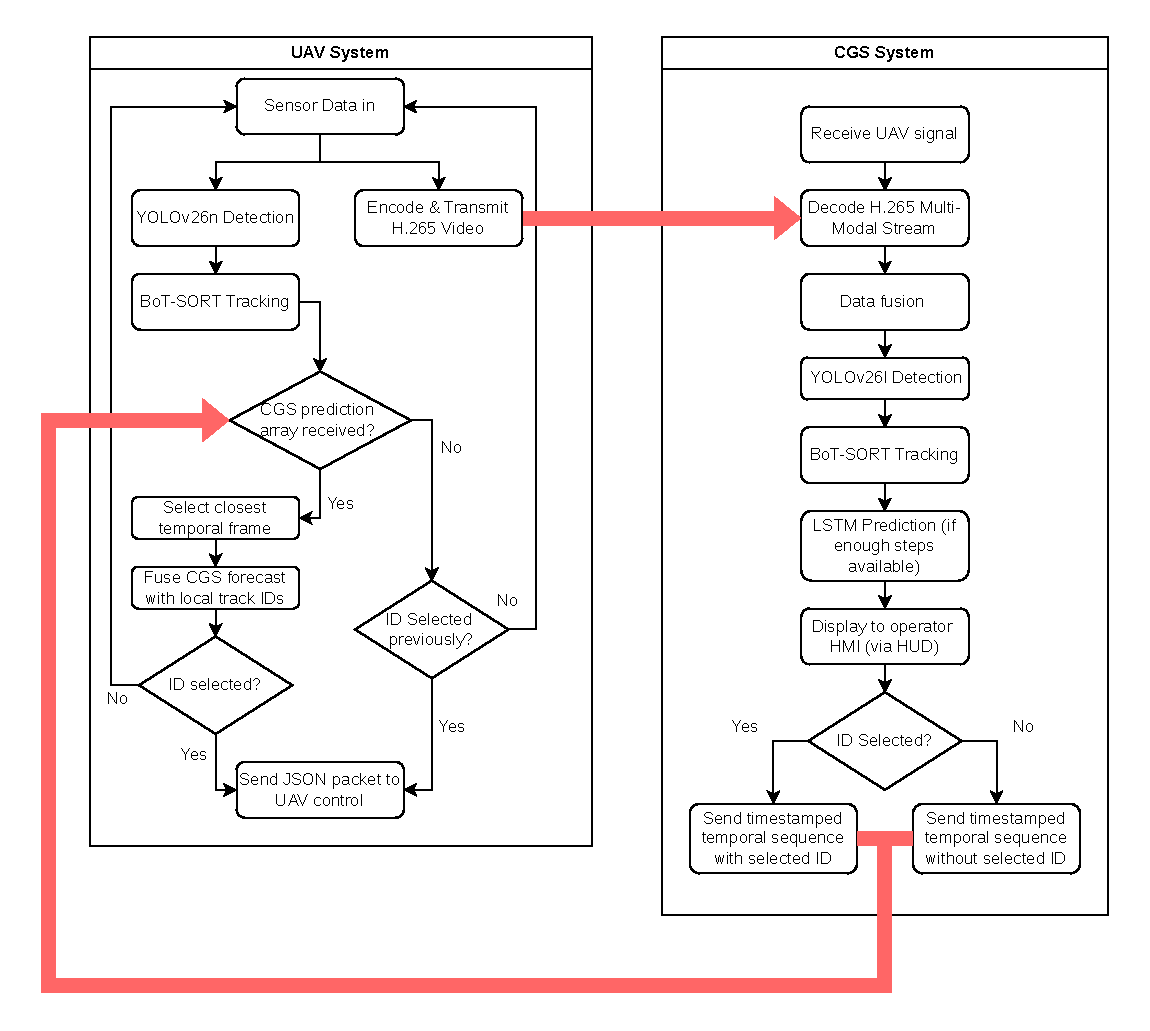
\includegraphics[width=1\linewidth]{figs/predictive_compensation_diagram.pdf}
    \caption{System Flowchart}
    \label{fig:predictive_compensation_diagram}
\end{figure}

The combined  edge-cloud system aims to carry out detection and tracking independently and merge them locally on the drone, using the \gls{cgs} message as a parent. Since the \gls{rtt} is calculated as approximately 150ms in [Hardware] and the system aims to run at 20 \gls{fps}, the \gls{lstm} predicts 2-6 frames ahead of its input multi-modal data feed to account for fluctuations in communication latency, which is then transmitted as a \textbf{timestamped temporal sequence}. The drone can then select the closest temporal frame before merging. If there is an existing selected ID, then the target object coordinates is given to the drone control and path planning. 

\subsubsection{C2 Telemetry Bandwidth Constraints}
A critical constraint of the distributed \gls{pads} architecture is the 115 kbps (14.37 KB/s) bandwidth limit of the sub-GHz C2 telemetry link (Section 3.3). If the \gls{cgs} transmitted the standard MOT16 sequence format for all maximum expected background targets (40 objects at 20 FPS, forecasting 4 frames ahead), the system would generate 3,200 entries per second. At approximately 15 bytes per ASCII string, this requires 384 kbps, catastrophically exceeding the radio's hardware limits. 

To resolve this bandwidth bottleneck, the \gls{cgs} implements a dynamic routing protocol based on operator \gls{hmi} selection. When no specific suspect is selected, the \gls{cgs} transmits global tracking data at a heavily down-sampled rate (2 Hz) to passively update the edge model's background IDs. However, once the operator selects a specific target ID, the \gls{cgs} isolates that singular trajectory forecast. Transmitting 4 forecasted frames for a single target at 20 FPS generates only 80 entries per second (1.2 KB/s, or 9.6 kbps), consuming less than 10\% of the available C2 bandwidth while ensuring zero-latency predictive compensation for the active pursuit.


\subsection{Heads-Up Display} \label{hud}
To ensure a police operator can make rapid, informed decisions, the drone’s local perception, BoT-SORT \cite{botsort} tracking, and \gls{cgs} predictive compensation are integrated concisely into a single \gls{hud}. Real-time detections are visualised via standard green bounding boxes, with the operator's selected target explicitly highlighted. Global situational awareness is maintained via an active object counter located in the top-left quadrant of the display.

Crucially, the architecture's temporal forecasting is rendered directly onto the tracked target. As demonstrated in Figure 4, the LSTM's calculated trajectory is depicted via a yellow vector arrow originating from the target's current center point, ending at a red dot representing the predicted spatial location. This allows operators to visually verify the \gls{lstm}'s forecast in real-time.

\begin{figure}[H]
    \centering
    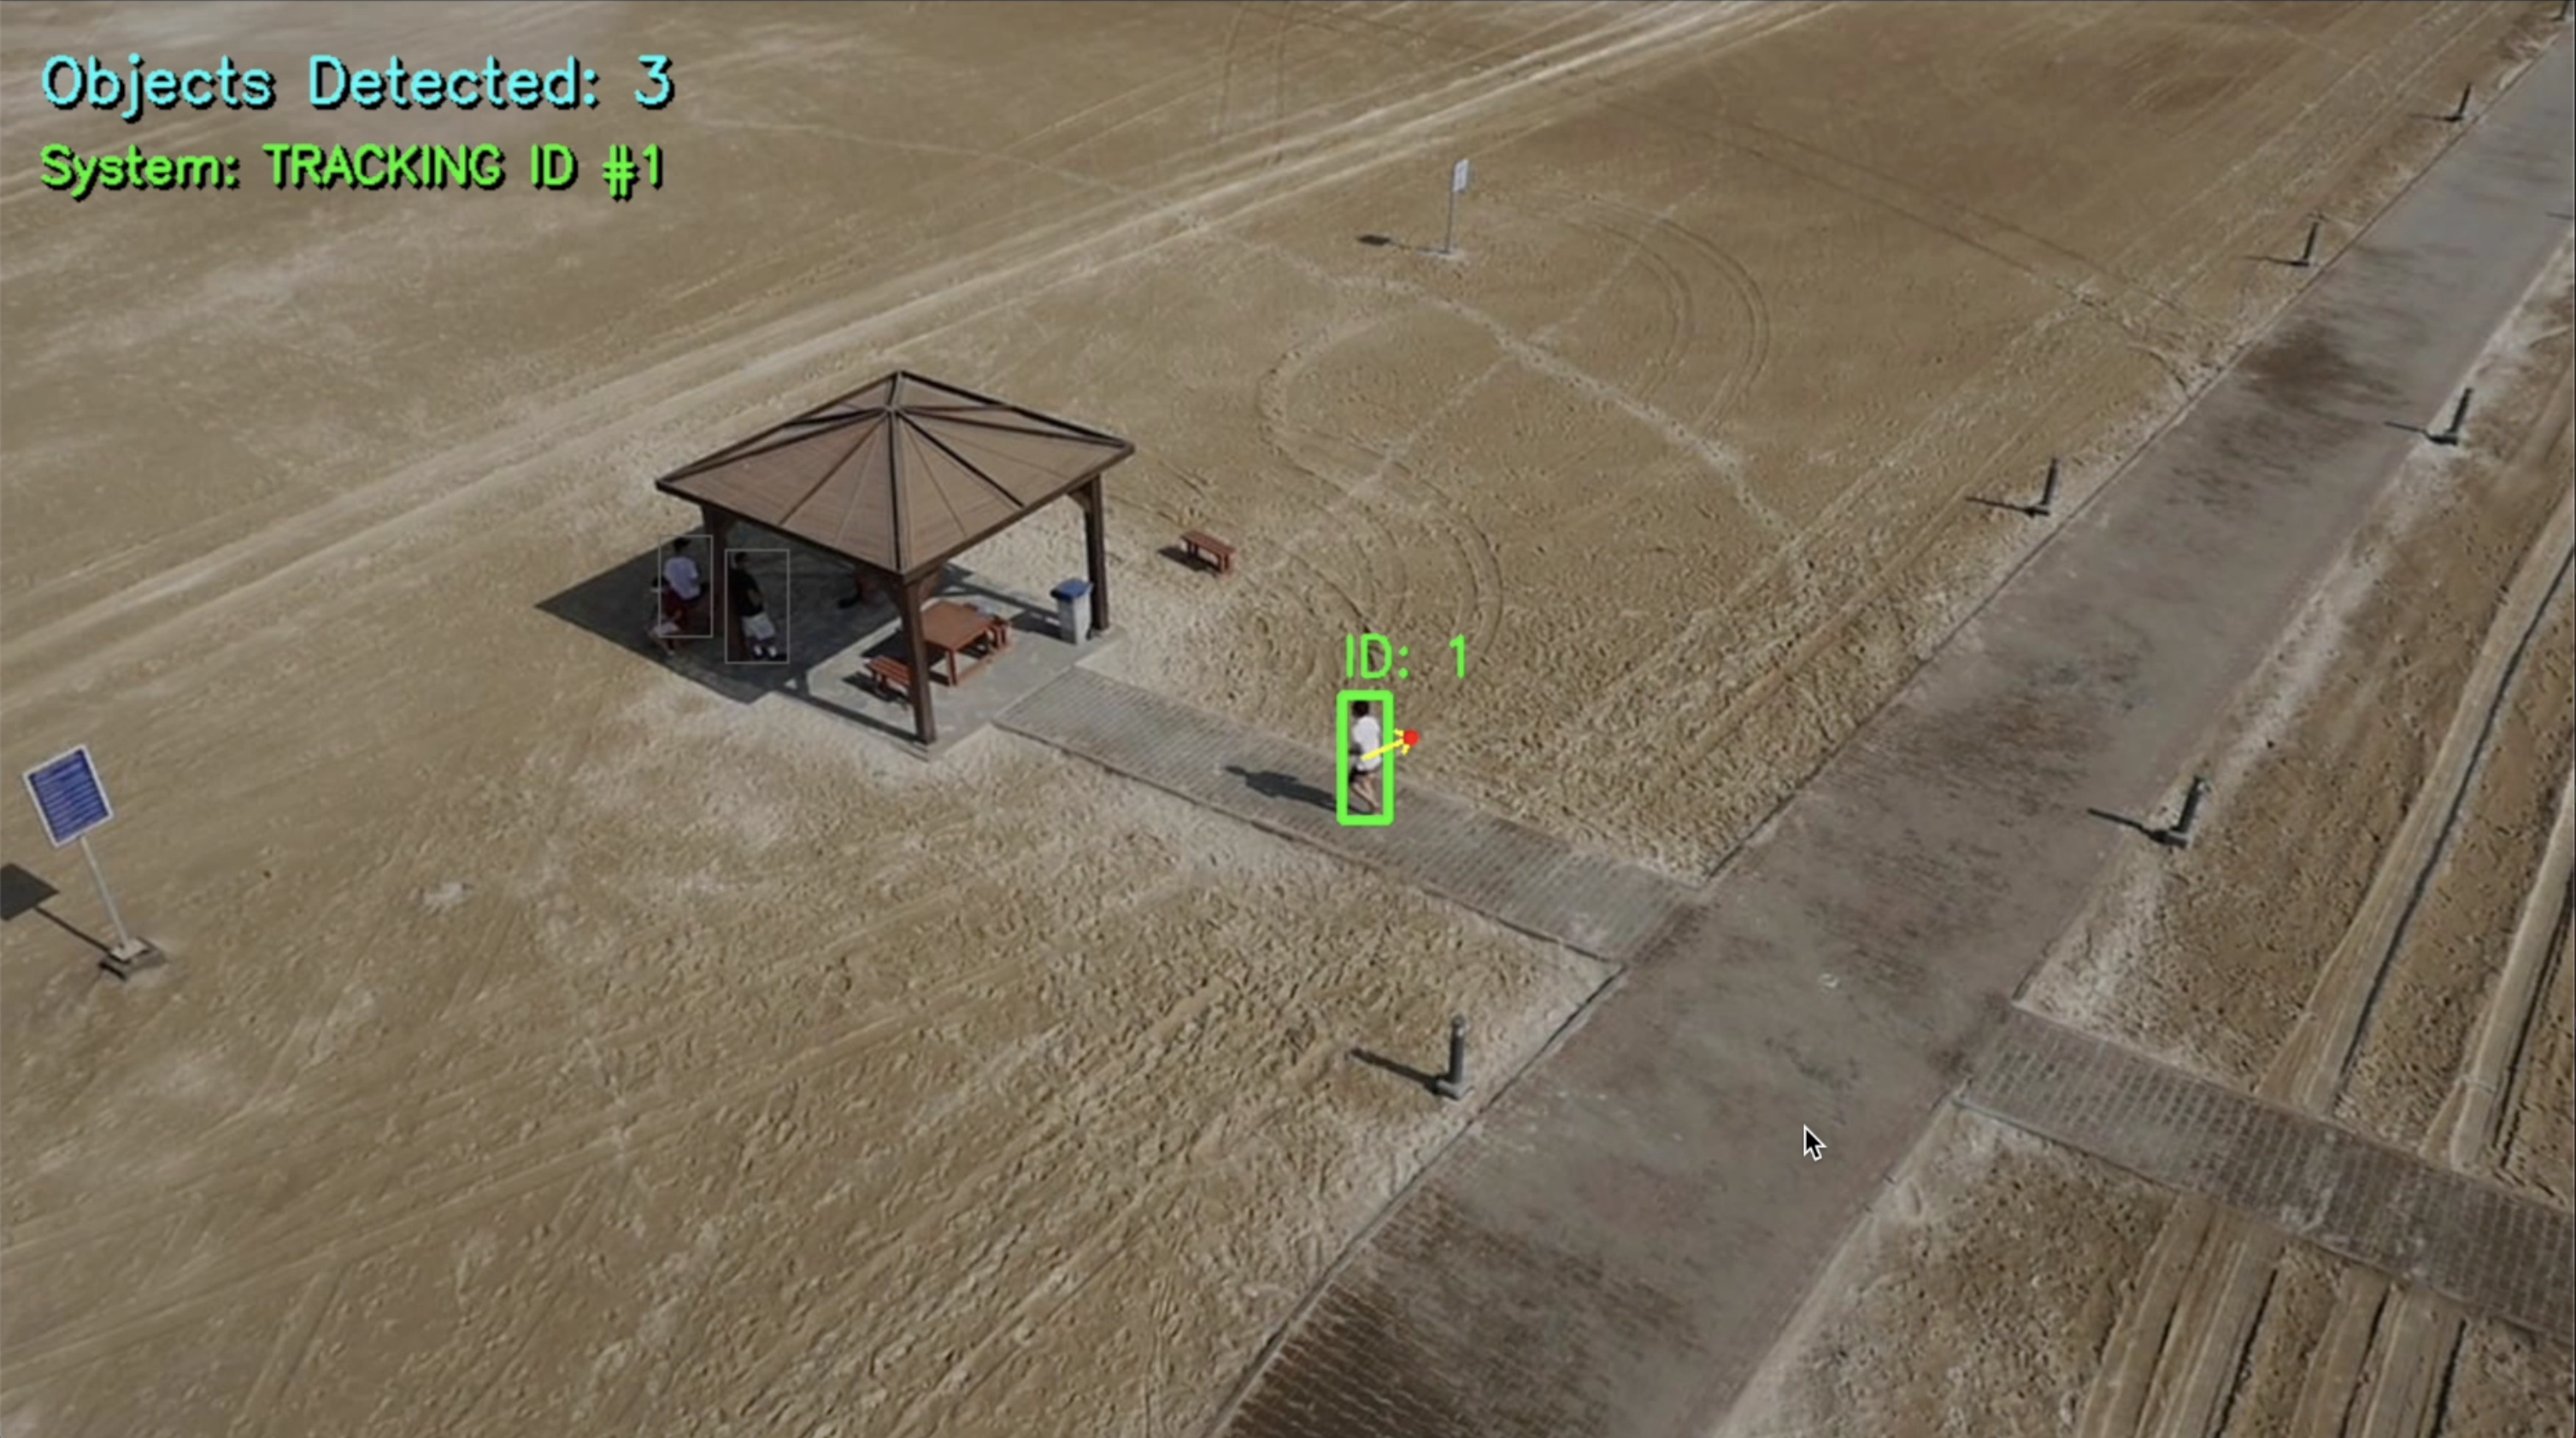
\includegraphics[width=1\linewidth]{figs/HUD.png}
    \caption{HUD implementation}
    \label{fig:placeholder}
\end{figure}

\printbibliography{3YP}

% Appendix
% Essential content that interrupts the flow of the document can be placed here, e.g. technical drawings, detailed lists of equations used, etc.
\newpage
\addcontentsline{toc}{section}{Appendix}
\section*{Appendix}

\end{document}
